%!TEX root = ../bare_adv.tex
\subsection{Introduction}
When talking about indoor positioning, a Graph-based Model~\cite{Jensen:2009:GMB:1590953.1591000} describes the topology of e.g. a floor plan of the indoor area. 
This area may be a complex area with several rooms, levels, doors, hallways etc. 
The Graph-based Model therefore represents the connectivity and accessibility of the area, representing each room as a vertex and each connection as an edge. 

By representing the area using a Graph-based Model, it is possible to apply indoor tracking of the people that are inside the area, using various wireless technologies (like bluetooth, Wi-Fi, RFID etc.) by logging the movement of the people or objects we want to track.

%A Graph-based Model can be applied, as it does not differ between the actual floor plan and the abstract model, hence why using an abstract model provides a equally correct positioning data. 

\subsection{Explained}
There are two kinds of Graph-based Models that describes the the topology of a floor plan. 
The first is the Connectivity Graph which describes how rooms, hallways, stairs etc. are connected to each other. 
The second is the Accessibility Graph which takes the actual accessibility of a cell into account. 
These two will be described in the following sections. 


\subsubsection{ \quad Connectivity Graph}
Both the Connectivity graph and the Accessibility Graph are based on a base-graph, which is constructed based on the actual floor plan. 

\begin{figure}[H]%
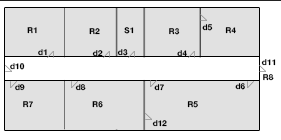
\includegraphics{images/floorplan.png}%
\caption{Floor plan of a building. Inspired from~\cite{Jensen:2009:GMB:1590953.1591000}}%
\label{fig:floortplan}%
\end{figure}%

Figure \ref{fig:floortplan} shows the floor plan that forms the basis of the examples of the Connectivity graph and the Accessibility graph. 
It contains 7 cells, labeled $R1 - R7$, one staircase labeled $S1$, a hallway and 12 doors labeled $d1-d12$. \\

In the Connectivity graph, each separate partitioning of the floor plan (rooms, staircases, hallways etc.) are represented as vertices, while the connectivity of these (doors, windows, hatches etc.) are represented as the edges.
E.g. if two rooms are connected by a door, each cell will be represented in the base-graph as a vertex, while the door is represented as an undirected edge. 
The Connectivity graph representing the floor plan in Figure \ref{fig:floortplan} is shown in Figure \ref{fig:connectivitygraph} below. 

\begin{figure}[H]%
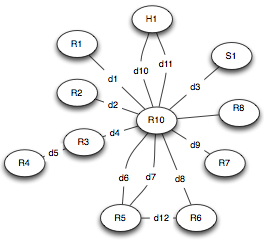
\includegraphics{images/connectivitygraph.png}%
\caption{Connectivity Graph of the floor plan in Figure \ref{fig:floortplan}.}%
\label{fig:connectivitygraph}%
\end{figure}%

Figure \ref{fig:connectivitygraph} shows how the rooms and hallways in Figure \ref{fig:floortplan} are connected by doors. 
The Connectivity graph itself is a labeled, undirected multi-graph that is defined by the following triple: \\

\begin{equation}
G_{connection} = (V, E_d, \Sigma_{door})
\end{equation}
In this triple, $V$ is the set of vertices in in the Graph. 
$E_d$ is the set of edges in the Graph, where any edge in $E_d$ is a pair consisting of $({v_i, v_j}, k)$ such that $v_i, v_j \in V$ and $k \in \Sigma_{door}$.
Finally, $\Sigma_{door}$ is a set of edge labels that represent the connections. 

However, it does not make much sense to look at the Connectivity Graph alone when talking about indoor positioning and tracking. 
To be able to track movement, information about the accessibility of each vertex must also be available. 

\subsubsection{ \quad Accessibility Graph}
There may be situations where a connection does not mean that you have access through that connection.
It can be air-port security or subway ententes that are either entries or exits, which allows one-way movement only.
To take this into account, the Accessibility graph is used. 
The Accessibility graph for the floor plan in Figure \ref{fig:floortplan} is shown in Figure \ref{fig:accesibbilitygraph} below.

\begin{figure}[H]%
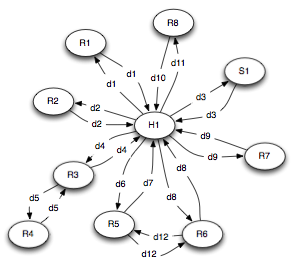
\includegraphics{images/accessibilitygraph.png}%
\caption{Accesibility graph of the floor plan in Figure \ref{fig:floortplan}.} % and the connectivity graph in Figure \ref{fig:floortplan}.}%
\label{fig:accesibbilitygraph}%
\end{figure}%

Figure \ref{fig:accesibbilitygraph} shows the accessibility graph..
It can be seen that door $d10$ only allows entrance from outside and into the Hall, while door $d11$ only allows exit from the Hall.
The Accessibility graph is a labeled, directed graph and constructed to represent possible movement patterns in the area. \\

An Accessibility graph named $G_{access}$ is given by the triple: 

\begin{equation}
G_{access} = (V, E, \Sigma_{door}, l_e)
\end{equation} 

where $V$ is the set of vertices, $E$ is the set of directed edges, having $E = \{\langle v_i, v_j \rangle | v_i, v_j \in V,  v_i \not= v_j\}$ and finally $l_e$ is a function that maps edges to subsets of the doors, having $l_e : E \rightarrow 2^{\Sigma_{door}}$. \\

These graphs provide an abstract representation of the floor plan, which -- combined with the previously mentioned logging -- will allow for indoor movement tracking and indoor positioning. 

%\IEEEPARstart{T}{his} demo file is intended to serve as a ``starter file''
%for IEEE Computer Society journal papers produced under \LaTeX\ using
%IEEEtran.cls version 1.7 and later.
% You must have at least 2 lines in the paragraph with the drop letter
% (should never be an issue)
%I wish you the best of success.
%\hfill mds
%\hfill January 11, 2007
